\documentclass[11pt]{article}

\usepackage{amssymb,amsmath,amsthm}
\usepackage{verbatim}
\usepackage{fullpage}
\usepackage{gencor}
\usepackage{mathrsfs}
\usepackage{authblk}
\usepackage{graphicx}
\usepackage{caption}
\usepackage{subcaption}
\numberwithin{equation}{section}
\usepackage[nottoc,notlof,notlot,numbib]{tocbibind}
\usepackage{xr-hyper}
\externaldocument[supp-]{supp}

\frenchspacing

\title{Estimating Genetic Correlations between Traits from GWAS Summary Statistics}
\author{Brendan Bulik-Sullivan*, Hilary Finucane*, ... , \emph{et. al.}}

\begin{document}
\maketitle

\newpage
\tableofcontents
\listoffigures
\listoftables
\newpage





%%%%%%%%%%%%%%%%%%%%%%%%%%%%%%%%%%%%%%%%%%%%%%%%%%%%%%%%%%%%%%%
\section{Introduction}
\label{Introduction}
%%%%%%%%%%%%%%%%%%%%%%%%%%%%%%%%%%%%%%%%%%%%%%%%%%%%%%%%%%%%%%%

Discovering relationships between phenotypes is a fundamental goal of epidemiology,
with applications to drug development, classification and treatment of disease.
The traditional strategy has been to search for correlations between phenotypes via large observational epidemiological studies;
however the interpretation of results from these studies 
can be confounded by social factors that are difficult to control for.
An alternative strategy that is robust to confounding by social factors is to search instead for pairs of phenotypes with
shared genetic etiology. 

The largest currently available sources of genotype-phenotype data are genome-wide association studies (GWAS).
GWAS have identified tens of thousands of phenotype-SNP associations in total, but these associations are spread across
hundreds of phenotypes. 
At current sample sizes, the number of associated loci per phenotype is usually only in the tens to hundreds, since for most traits,
the majority of the genetic contribution to phenotypic variance is accounted for by variants with small effects, which cannot 
be confidently associated except with very large sample sizes.
Therefore, simply scanning for pairs of phenotypes with shared genome-wide significant loci is not a powerful approach for polygenic phenotypes.

A more powerful option is to use information from all genotyped SNPs to estimate the genome-wide 
(narrow-sense) genetic correlation between phenotypes;
however, existing methods for estimating genetic correlation from GWAS data,
such as restricted maximum likelihood (REML) as implemented in the software package GCTA 
\cite{yang2010, yang2011gcta, lee2012estimation}
require individual genotype and phenotype data, which can be difficult or impossible to obtain due to restrictions on data sharing.
For this reason, only a few dozen genetic correlations have been estimated from GWAS data to date 
\cite{pgccdg2013, vattikuti2012heritability, chen2014estimation}.

In this paper, we describe a method based on LD Score regression
which bypasses data sharing difficulties by estimating genetic correlations using only GWAS summary statistics.
These estimates extend the understanding gleaned from the handful of previously estimated
genetic correlations, giving us a big-picture view of how phenotypes cluster together as well as allowing 
us to skim for surprising and interesting genetic correlations.

In addition, we describe methods for relaxing some of the unrealistic assumptions about genetic architecture made by 
existing methods for estimating genetic correlation, 
and demonstrate that our method is minimally confounded  
when effect size depends on allele frequency or linkage disequilibrium.
As a sanity check, 
we replicate the genetic correlations reported by the PGC Cross-Disorder Group using REML in \cite{pgccdg2013},
using only the summary statistics from \cite{cross2013identification}.

Since dozens of sets of summary statistics can be freely downloaded from the internet,
we are able report a much larger number of genetic correlations 
 -- more than 300 mostly novel results in this paper alone -- than was previously possible.
Most genetic correlations tend to cluster within previously defined phenotypic categories;
however, we observe several surprising results that would have been difficult to obtain without methods that operate on summary statistics.

The computational demands of our method are very mild. 
If $N$ denotes sample size and $M$ denotes the number of SNPs, then LD Score regression takes
$\mathscr{O}(MN)$ time for computing summary statistics and $\mathscr{O}(M)$ time for the regression. 
For comparison, REML takes time $\mathscr{O}(MN^2)$ for computing the genetic relatedness matrix (GRM)
and $\mathscr{O}(N^3)$ time for maximizing the likelihood.
Practically, LD Score regression takes a matter of minutes on a standard laptop.
We provide an open-source software package, \texttt{ldsc},
written in python, which implements the analyses described in this paper and also the analyses from
\cite{buliksullivan2014, finucane2014partitioning} (URLs).


%%%%%%%%%%%%%%%%%%%%%%%%%%%%%%%%%%%%%%%%%%%%%%%%%%%%%%%%%%%%%%%
\section{Results}\label{Results}
%%%%%%%%%%%%%%%%%%%%%%%%%%%%%%%%%%%%%%%%%%%%%%%%%%%%%%%%%%%%%%%

\subsection{Overview of Methods}

The additive genetic covariance, $\rho_g$ between two phenotypes $y_1$ and $y_2$ is the bivariate analogue of heritability,
and is defined as the covariance (in the population) between the additive genetic components of $y_1$ and $y_2$. 
The normalized version of genetic covariance is genetic correlation,
\begin{equation}\label{gencov}
	r_g := \dfrac{\rho_g}{\sqrt{h^2_1h^2_2}},
\end{equation}
where $h^2_i$ denotes the heritability of trait $i$; genetic correlation lies in the interval $[-1,1]$.

The genetic correlation parameter that we estimate in this paper is different from the quantity estimated by family studies.
We focus on the narrow-sense (\emph{i.e.,} additive) genetic correlation among common SNPs; 
family studies attempt to estimate the total narrow sense genetic correlation.

Unlike the distinction between $h^2_g$, $h^2$ and $H^2$, where we have the inequality
$h^2_g < h^2 < H^2$,
no such inequality holds in general for the narrow-sense genetic correlation among SNPs, the total narrow-sense genetic
correlation and the broad-sense genetic correlation.

We can estimate the denominator of equation \ref{gencov} from summary statistics using single phenotype LD Score regression
as described in \cite{buliksullivan2014}.
In this paper, we describe a method for estimating of the numerator based off a simple modification
of the regression from \cite{buliksullivan2014}. 
Instead of regressing $\chi^2$-statistics against LD Score, we regress the product of $Z$-scores from two different GWAS
against LD Score, and the slope times a constant gives us an estimator of genetic covariance (Online Methods).

One major concern when estimating genetic correlations from GWAS summary statistics is that many pairs of GWAS
share large numbers of overlapping samples, so the $Z$-scores from one study may not be independent of the $Z$-scores
from another study even if the genetic correlation between the phenotypes studied is zero.
This turns out not to be a difficulty for LD Score regression. 
Since sample overlap affects all SNPs equally, sample overlap merely inflates the LD Score regression intercept,
and does not affect the slope (Supplementary Note).
If the amount of sample overlap and the phenotypic correlation among overlapping individuals is known ahead of time,
then it is possible to reduce the standard error of the genetic covariance estimate by constraining the intercept (Online Methods).
In addition, because LD Score is minimally correlated with $F_{ST}$ \cite{buliksullivan2014},
the LD Score regression estimator of genetic covariance is protected from shared population stratification.


\subsection{Simulations}\label{Simulations}
In order to check our derivations and verify the robustness of our inference procedure to 
violations of our modeling assumptions, we performed a variety of simulations. 


\subsubsection{Shared Population Stratification}

Shared population stratification is a potential confounder for estimates of genetic correlation.
For example, if a GWAS for phenotype one is confounded by population stratification from North/South European ancestry and the 
same is true of a GWAS for phenotype two, then the estimate of genetic correlation obtained from REML will be 
biased upwards 

Two-phenotype LD Score regression should on expectation be protected from from shared population stratification for exactly the 
same reasons that single phenotype LD Score regression is protected from shared population stratification \cite{buliksullivan2014}:
LD Score is essentially uncorrelated with $F_{ST}$, so shared population stratification will only inflate the intercept 
of the two-phenotype LD Score regression.

To verify this conclusion, we simulated pairs of phenotypes from real genotype under an additive model, then added an 
environmental stratification component to aligned with the first principal component 
of the genotype data to both phenotypes in each pair.
\textbf{INSERT RESULTS}

\subsubsection{Misspecified Models of Genetic Architecture}\label{Misspecified Sims}

Estimates of heritability and genetic covariance can be biased if the underlying model of genetic architecture is misspecified.
For example, Speed, \emph{et. al.} \cite{speed2012improved} 
demonstrate that REML can be confounded by MAF- or LD-dependent genetic architectures.
Lee, \emph{et. al.} (\cite{lee2013estimation}) showed that it is possible to correct for such biases using MAF-binned REML.
One can take a similar approach with LD Score regression to obtain unbiased estimates of heritability and genetic 
covariance even under MAF or LD-dependent genetic architectures (see \cite{finucane2014partitioning} and Online Methods).
Estimates of genetic correlation are more robust to model misspecification biases than estimates of heritability or genetic covariance.
Since genetic correlation is estimated as a ratio,
model misspecification biases that affect the numerator and the denominator in the same direction will tend to cancel. 

To quantify the bias introduced by MAF- or LD-dependent genetic architectures, we performed a series of simulations,
using a variety of different LD Scores and genetic architectures.
In order to simulate the realistic scenario where only a subset of causal SNPs are directly genotyped,
we used a densely imputed panel of 1000 Genomes (1kG) SNPs \cite{10002012integrated} in order to generate phenotypes
and estimate LD Scores, 
but computed summary statistics only for HapMap3 (HM3) SNPs \cite{international2010integrating}
Results from these simulations are displayed in Supplementary Tables 
\ref{supp-parallel}, \ref{supp-antiparallel} and \ref{supp-depcor}.

We found that the binned LD Scores were almost completely immune to MAF- and LD-dependent genetic architectures
when estimating heritability and genetic covariance, but gave substantially higher standard errors.
The simplest LD Score model, with LD Scores computed using only ``genotyped'' SNPs (\emph{i.e.,} HM3 SNPs)
 -- hereafter referred to as 
HM3 LD Score --  was the best performing estimator of genetic correlation. 
Estimates of genetic correlation from this model had the lowest standard error, and
were unbiased in simulations where heritability and genetic covariance depended on LD, 
with only minimal bias even in simulations where genetic correlation also depended on LD.  

In all of the simulations described in this section, 
there was full sample overlap, which confirms that the LD Score regression estimator of 
genetic correlation is not biased by sample overlap.


%%%%%%%%%%%%%%%%%%%%%%%%%%%%%%%%%%%%%%%%%%%%%%%%%%%%%%%%%%%%%%%
\subsection{Real Data}\label{Real Data}
%%%%%%%%%%%%%%%%%%%%%%%%%%%%%%%%%%%%%%%%%%%%%%%%%%%%%%%%%%%%%%%

\subsubsection{Replication of PGC Cross Disorder Results}\label{PGCCDG}

For further validation, we replicated the estimates of genetic correlations between psychiatric phenotypes obtained with
individual genotypes and REML in the PGC Cross-Disorder Group paper \cite{pgccdg2013}, 
using LD Score regression and the summary statistics from \cite{cross2013identification},
downloaded from the PGC website (URLs).
Since the HM3 LD Score was the best-performing estimator of genetic correlation in simulations, 
we used this LD Score for application to real data. 

Including an intercept in the LD Score regression protects the results from QC issues such as population stratification (as described in \cite{buliksullivan2014})
and sample overlap, but at the cost of a substantial increase in standard error.
Since the summary statistics from \cite{cross2013identification} were generated after a careful QC process, and the 
samples used for each disease were non-overlapping, we also fit LD Score regression with constrained intercepts \cite{buliksullivan2014he}.

Results from this analysis are displayed in Figure \ref{Fig:Replication of PGC Cross Disorder Results}.
As expected, the genetic correlation estimates from LD Score regression with HM3 LD Scores were very similar to the results from REML.
LD Score regression without intercept gave standard errors that were only slightly larger than REML,
while the standard errors from LD Score regression with intercept were somewhat larger, especially for the very small studies
(\emph{e.g.,} ADD, Autism).

The computational demands of this analysis were trivial: after computing LD Scores and pre-processing the summary statistics, 
the LD Score regression took about one minute per pair of phenotypes
(most of which was spent reading compressed LD Score files into memory) 
and less than 1GB of RAM. 

\begin{figure}[!ht]

\begin{centering}
\caption{Replication of PGC Cross Disorder Results}
    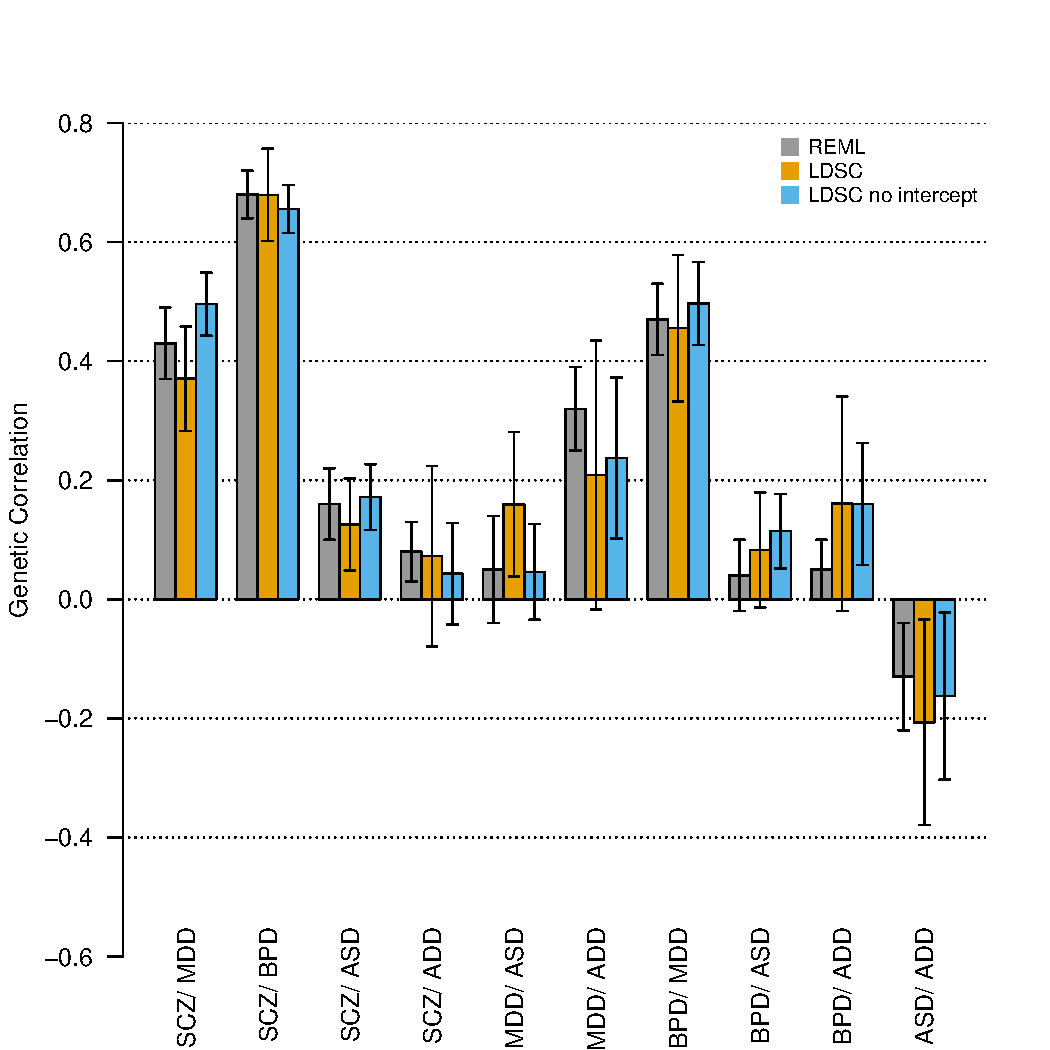
\includegraphics[scale=0.8]{figs/ldsc_vs_gcta.pdf}
         \label{Fig:Replication of PGC Cross Disorder Results}

\end{centering}

\small{\textit{This plot compares LD Score regression estimates of genetic correlation using the summary statistics from \cite{cross2013identification} (which were generated from approximately the same data as \cite{pgccdg2013}) to 
estimates obtained from REML in \cite{pgccdg2013}.
The horizontal axis indicates pairs of phenotypes, and the vertical axis indicates genetic correlation.
Colors indicate different estimation procedures. Grey is REML,
Orange is HM3 LD Score with intercept; blue is HM3 LD Score without intercept, 
The estimates of genetic correlation between psychiatric phenotypes presented under the header 
``Application to a Large Set of Publicly Available Summary Statistics" use larger sample sizes, and so are more reliable;
this plot is intended primarily as a technical sanity check.
Abbreviations: 
ADD = Attention Deficit Hyperactivity Disorder (1947 trio cases, 1947 trio pseudocontrols, 840 cases, 688 controls);
ASD = Autism Spectrum Disorder (4788 trio cases, 4788 trio pseudocontrols, 161 cases, 526 controls);
BPD = Bipolar Disorder (6990 cases, 4820 controls);
MDD = Major Depressive Disorder (9227 cases, 7383 controls);
SCZ = Schizophrenia (9379 cases, 7736 controls).}}

\end{figure}

\subsubsection{Application to a Large Set of Publicly Available Summary Statistics}
We applied our method to 27 publicly available sets of GWAS summary statistics,
including   
schizophrenia \cite{schizophrenia2014biological}, 
major depression \cite{ripke2012mega}, 
bipolar disorder \cite{sklar2011large}, 
autism \cite{cross2013identification},
attention-deficit hyperactivity disorder \cite{neale2010meta},
anorexia \cite{boraska2014genome},
height \cite{allen2010hundreds}, 
body mass index \cite{speliotes2010association}, 
BMI-adjusted waist-hip ratio \cite{heid2010meta}, 
obesity \cite{berndt2013genome}, 
fasting glucose
\cite{manning2012genome},
HOMA-B,
HOMA-IR \cite{dupuis2010new},
HbA1C \cite{soranzo2011genetic},
cigarettes per day,
age of onset of smoking,
ever vs never smokers,
former vs current smokers \cite{tobacco2010genome},
coronary artery disease \cite{schunkert2011large}, 
type-2 diabetes \cite{morris2012large}, 
rheumatoid arthritis \cite{stahl2010genome}, 
high-density lipoprotein,
low-density lipoprotein,
triglycerides,
total cholesterol \cite{teslovich2010biological},
ulcerative colitis \cite{jostins2012host},
Crohn's disease \cite{jostins2012host} and 
Alzhiemer's disease \cite{lambert2013meta}
(see URLs for a full list of links).
   
Because HM3 LD Score performed best in simulations, we used this LD Score for estimating all pairwise genetic correlations.
The majority of these studies share some samples, so we did not constrain any of the LD Score regression intercepts.
The subset of genetic correlation estimates that were statistically significantly different from zero after correction for 351 
tests at 5\% false discover rate (FDR) are displayed as a heatmap in Figure \ref{Fig:300 Gencors}.
The full set of genetic correlation estimates are provided in tabular (\texttt{csv}) format in the Supplementary Data.

\begin{figure}[!ht]

\begin{centering}
\caption{Genetic Correlations Between 27 Published GWAS}
    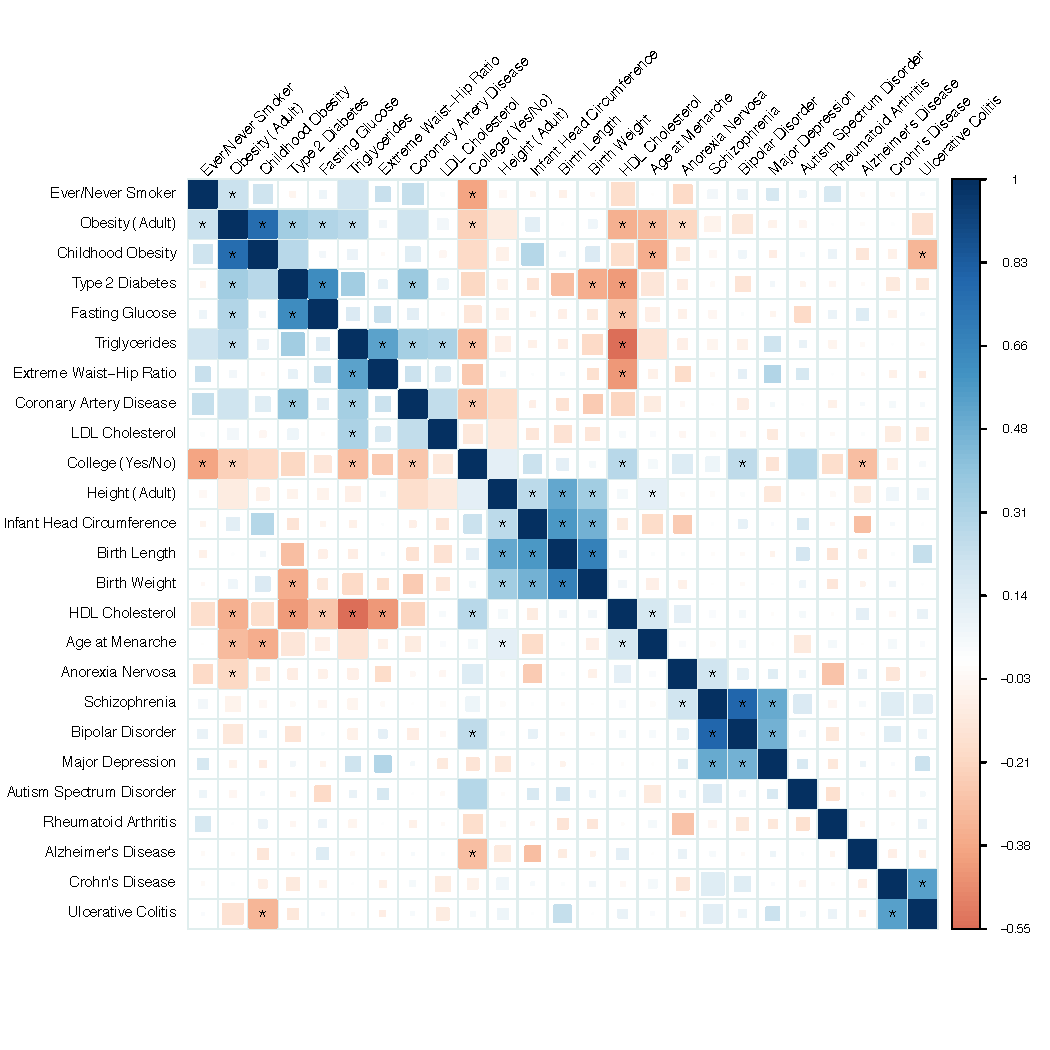
\includegraphics[scale=1]{figs/rg_heatmap.pdf}
         \label{Fig:300 Gencors}

\small{\textit{This figure displays genetic correlations between the 27 phenotypes analyzed estimated with HM3 LD Score. 
The genetic correlations are color coded according to sign and magnitude.
Only the genetic correlations that are statistically significantly different from zero at an FDR of 0.05 are displayed;
the rest have been whited out.}}

\end{centering}
\end{figure}
We find that phenotypes tend to cluster into categories defined by clinical practice and observational epidemiology;
for instance, we observe high genetic correlations between anthopometric traits, between psychiatric traits,  between 
metabolic traits and between autoimmune traits.
Reassuringly, most genetic correlations across pre-defined phenotypic categories were within not significantly different from
zero.

Our results on genetic correlation between metabolic traits are generally consistent with the results from 
\cite{vattikuti2012heritability}, though our standard errors are lower by an order of magnitude, since operating on summary statistics
allows us access to far larger sample sizes (Supplementary Table \ref{supp-vattikuti}). 
The only discrepancies came from waist-hip ratio (WHR). 
The data that we used were from a GWAS for BMI-adjusted WHR \cite{heid2010meta}; whereas
Vattikuti \emph{et. al.} use unadjusted WHR. 
These are very different phenotypes, 
so it is unsurprising that their genetic correlation profiles differ (Supplementary Table \ref{supp-whr}).
In addition, our estimate of the genetic correlation between Crohn's disease and ulcerative colitis (0.57 SE 0.063) is consistent
with the estimate from \cite{chen2014estimation} (0.62 SE 0.042).



\textbf{SUGGESTED COOL EXAMPLES}
\begin{enumerate}

	\item smoking traits all have near total rg despite no shared gwsig SNPs (goes against the interpretation offered by TAG)
	\item first ever SNP rg's for AN (BMI/SCZ have best p-values, replicate in PGC-AN)
	\item zero rg between alzheimers and psychiatric stuff
	\item alzheimers and height (Z = 9)???
	\item dense metabolic cluster at the top left
	\item CD/UC and SCZ \cite{benros2011autoimmune, benros2014nationwide}
	\item 0 rg for SCZ and RA (though a small effect may be meaningful, and we are not well-powered to detect anything between 		0 and -0.1)
\end{enumerate}



\subsection{Heritability}

The majority of the summary statistics that we analyzed were ``corrected'' via genomic control correction. 
GC correction is both ineffective at correcting for population stratification \cite{price2006principal},
and excessively conservative \cite{buliksullivan2014}.
As a result, an increasing number of recent meta-analyses have opted not to employ GC correction
\cite{jostins2012host, ripke2012mega, neale2010meta, sklar2011large, schizophrenia2014biological, wood2014defining}
In addition, LD Score regression estimates of heritability and genetic covariance from GC corrected summary statistics are biased
downwards
\cite{buliksullivan2014} 
(the genetic correlation estimates are not biased, because the multiplicative bias in the numerator 
and the multiplicative bias in the denominator cancel exactly). 
Thus, we can only present heritability estimates for the subset of GWAS that did not use GC correction.

We had information on sample MAF and imputation quality for schizophrenia, CD and UC,
so we used all 1kG SNPs with sample MAF above 3\% and INFO above 0.9 for these LD Score regressions, 
since using a larger set of SNPs or the regression decreases the standard error.   
We estimated heritability using LD Scores partitioned on derived allele frequency (DAF) and LD Score, to account for possible DAF-
or LD-dependence in genetic architecture (Online Methods),
both with and without constraining the LD Score regression intercept to equal one. 
Heritability estimates for UC, CD, SCZ and BPD are displayed in Table \ref{Table:h2}.
\begin{table}[t]
\centering
\caption{Heritability Estimates}
\label{Table:h2}
\begin{tabular}{rllll}
  \hline
\input{./table/h2}
\end{tabular}

\small{\textit{Liability scale heritability estimates for CD, UC, SCZ and BPD.
The first row contains estimates of $h^2_{5\myhyphen50\%}$ from LD Score regression with intercept constrained to one.
The second row contains estimates of $h^2_{5\myhyphen50\%}$ from LD Score regression with unconstrained intercept.
The LD Score regressions for CD, UC and SCZ used approximately 6 million well-imputed (INFO $>$ 0.9) 1kG SNPs. 
The LD Score regression for BPD used 1.2 million HM3 SNPs since this GWAS did not use 1kG imputation.
All LD Score regressions in this table used a DAF $\times$ LD Score partitioned LD Score regression model with 35 bins. 
The estimates of $h^2_g$ for CD and UC are from \cite{chen2014estimation}; 
the estimates of $h^2_g$ for SCZ and BPD are from \cite{pgccdg2013}.
The prevalence row contains the population prevalences used for transformation to the liability scale. 
Estimates of liability scale heritability should be interpreted cautiously, since for many diseases,
estimates of prevalence are fuzzy.}}
\end{table}


We also display estimates of $h^2_g$ from earlier publications, 
though we caution that $h^2_g$ and $h^2_{5\myhyphen50\%}$ are not the same quantity,
so any comparison between them is technically
apples-to-oranges (see Section \ref{h2550} in the Methods).
The estimates of $h^2_g$ in Table \ref{Table:h2} were obtained using REML on ascertained samples, 
and so may be biased downwards \cite{golan2013narrowing, chen2014estimating}.
The heritability estimates with constrained intercept differed from the estimates with unconstrained intercept by less than one
standard error in all cases except for UC, where the difference was substantial. 
This could be explained either 
by a small amount of residual population stratification in the summary statistics (even after careful QC), 
reference/target LD mismatch or model misspecification bias not fully accounted for by the partitioning. 


%%%%%%%%%%%%%%%%%%%%%%%%%%%%%%%%%%%%%%%%%%%%%%%%%%%%%%%%%%%%%%%
\section{Discussion}\label{Discussion}
%%%%%%%%%%%%%%%%%%%%%%%%%%%%%%%%%%%%%%%%%%%%%%%%%%%%%%%%%%%%%%%\

\subsection{Genetic Correlation is Different from Pleiotropy}

Genetic correlation is defined as the correlation across SNPs of additive per-normalized genotype effect sizes for two traits.
Pleiotropy is defined as the tendency for the same variants to have nonzero effects on two or more phenotypes. 
Genetic correlation is a strictly stronger condition than pleiotropy:
to exhibit genetic correlation, it is not sufficient for two phenotypes to be influenced by the same genetic variants,
the directions of effects must also be consistently aligned across the genome.

Nevertheless, both quantities are informative. 
If two phenotypes are influenced by variants at the same loci or in the same pathways, this may well indicate interesting
shared biology, even if the direction of the effects do not align. 
However, quantifying genome-wide pleiotropy from GWAS summary statistics remains an open challenge
\cite{solovieff2013pleiotropy}. 
For example, since $p$-values tend to decrease with LD Score \cite{buliksullivan2014} and near coding and regulatory
regions \cite{gusevregulatory}, the observation that low $p$-values for one phenotype tend to predict low $p$-values for another 
(as in \cite{schork2013all, andreassen2013improved, andreassen2013improved2})
may merely reflect properties shared by almost all pairs of heritable phenotypes, 
rather than a special property of a specific pair of phenotypes 
(Supplementary Figures \ref{supp-pleiotropy}, \ref{supp-qq_tg}, \ref{supp-qq_bip}).
Genetic correlation estimates from LD Score regression are not affected by these concerns, and so may be more 
easily interpretable than currently-available estimates of genome-wide pleiotropy.


\subsection{Limitations and Future Directions}

We note some limitations of LD Score regression and interpretation of estimates of genetic correlation from GWAS data
in general. 
First, LD Score regression requires large sample sizes (at least several thousand) in order to give estimates with reasonable
standard error. 
For smaller sample sizes, REML is a more statistically efficient estimator of genetic correlation when its assumptions
are met (in particular, for non-ascertained studies) and individual genotypes are available.

Second, LD Score regression assumes that all individuals in the GWAS were sampled from populations with similar LD Scores,
and that these LD Scores can be estimated from sequence data.
For multi-continental GWAS, the solution is to run LD Score regression on each continental subcohort separately, 
but nevertheless, LD Score regression can only be applied to samples from populations for which there exists a large 
sequenced reference panel. 
Currently, LD Score regression cannot be applied to samples from admixed populations.

Third, while genetic correlations are less confounded than overall phenotypic correlations from observational
epidemiology, genetic correlations cannot be interpreted as causal effects, even genetic correlations between intermediate 
phenotypes and disease.
For example, consider the strong negative genetic correlation between HDL and CAD in Figure \ref{Fig:300 Gencors}.
This genetic correlation could result from a causal effect, \emph{e.g.,} $\mathrm{HDL}\rightarrow\mathrm{CAD}$,
but could also result from non-causal shared genetic etiology 
\emph{e.g.,} $\mathrm{HDL}\leftarrow\mathrm{G}\rightarrow\mathrm{CAD}$, where $\mathrm{G}$ is some set of 
unknown genetic factors.
Indeed, the second explanation seems most likely in this case, because the genetic correlation between 
HDL and CAD has been observed to vanish after controlling for genetic correlations with other plasma lipids \cite{do2013common}.


Fifth, while LD Score regression is a consistent estimator of genetic correlation given samples where cases have been 
oversampled, it may be biased by misclassification of phenotypes or by more subtle forms of ascertainment. 
Thus, it is best to interpret estimation of genetic correlation from GWAS summary statistics as a hypothesis-generating 
exercise. 
This method allows us to screen hundreds of pairs of phenotypes with computational ease, but any findings
should be followed-up with confirmatory analyses, including a detailed review of the ascertainment procedures
in each GWAS.

Finally, it is impossible to obtain any estimates of genetic correlation at all unless researchers are willing to share full sets of GWAS 
summary statistics.
Since summary statistics contain such a large amount of information about genetic architecture and the relationships between 
phenotypes, it is surely the case that the benefits of data sharing outweigh the costs.
To facilitate data sharing, we have written a short guide describing the necessary information in Section \ref{Summary Statistics} of the Methods.

\subsection{Conclusion}

We have described a method for estimating common variant heritability and
genetic correlation that requires only GWAS summary statistics as input data.
Our method is immune to case/control ascertainment, sample overlap, shared population stratification \cite{buliksullivan2014}, 
and can be easily modified to be protected from bias from MAF- and LD-dependent genetic architectures. 
The computational demands of our method are mild: a few minutes on a standard laptop, irrespective of sample size.
Although LD Score regression does not use individual-level data,
the increase in standard error relative to methods that do use individual genotype and phenotype data is only moderate. 
In fact, LD Score regression without intercept is equivalent to HE regression \cite{buliksullivan2014he}.

...etc

\newpage
%%%%%%%%%%%%%%%%%%%%%%%%%%%%%%%%%%%%%%%%%%%%%%%%%%%%%%%%%%%%%%%
\section{Online Methods}\label{Online Methods}
%%%%%%%%%%%%%%%%%%%%%%%%%%%%%%%%%%%%%%%%%%%%%%%%%%%%%%%%%%%%%%%

%%%%%%%%%%%%%%%%%%%%%%%%%%%%%%%%%%%%%%%%%%%%%%%%%%%%%%%%%%%%%%%
\subsection{Statistical Framework}
%%%%%%%%%%%%%%%%%%%%%%%%%%%%%%%%%%%%%%%%%%%%%%%%%%%%%%%%%%%%%%%

See the supplementary note for a thorough derivation of the models behind LD Score regression.


%%%%%%%%%%%%%%%%%%%%%%%%%%%%%%%%%%%%%%%%%%%%%%%%%%%%%%%%%%%%%%%
\subsection{Definitions}\label{h2550}
%%%%%%%%%%%%%%%%%%%%%%%%%%%%%%%%%%%%%%%%%%%%%%%%%%%%%%%%%%%%%%%

\subsubsection{Heritability}

Let $S$ denote a set of $M$ SNPs, 
let $X$ denote the random $M$-vector of additively (0-1-2) coded genotypes for the SNPs in $S$, 
and let $y$ denote a phenotype. Define 
\begin{equation}
	\beta := \mathrm{argmax}_{\alpha\in\R^M} \corr\left[y, X\alpha\right]^2,
\end{equation}
where the maximization is performed in the population (\emph{i.e.,} at infinite sample size), rather than in a finite sample.
This is a projection, so uniqueness of $\beta$ is guaranteed as we remove SNPs that are linearly dependent (in the population). 
Then $h^2_S$, the heritability accounted for by SNPs in $S$, is defined
\begin{equation}\label{h2}
	h^2_S := \sum_{j=1}^M \beta_j^2.
\end{equation}
We obtain the Yang/Visscher parameter $h^2_g$ by taking $S$ to be the set of genotyped SNPs.
If we let $S$ denote the set of all SNPs in 1000 Genomes Europeans \cite{10002012integrated}, 
and let $S'$ denote the set of SNPs with MAF$>5\%$, then
\begin{equation}
	h^2_{5\myhyphen50\%} := \sum_{j\in S'} \beta_j^2.
\end{equation}
We choose 5\% as the lower bound, because we can estimate LD Scores for 5\% SNPs reasonably well from the $N=387$ 
samples in 1000 Genomes. 
Technically, we should write $h^2_{5\myhyphen50\%,1kG}$ to indicate that we are only accounting for SNPs in 1000 Genomes,
but 1000 Genomes has sufficiently good power to observe 5\% and higher SNPs that we feel justified in omitting 1kG from the subscript.
With larger sample sizes in future sequenced reference panels, this lower bound can be pushed lower.

There are two main distinctions between $h^2_{5\myhyphen50\%}$ and $h^2_g$,
First, $h^2_g$ does not include the effects of common SNPs that are not tagged by the set of genotyped SNPs $g$.
Second, the effects of causal 4\% SNPs are not counted towards $h^2_{5\myhyphen50\%}$.
In practice, neither of these distinctions makes a large difference, since most GWAS arrays focus on common variation
and manage to assay or tag almost all common variants.

Estimating $h^2_{5\myhyphen50\%}$ involves only as simple modification of LD Score regression: the raw slope from the 
regression divided by sample size yields an estimate of the average value of $\beta^2_j$. 
If we multiply this number by $M$, the number of SNPs in 1000 Genomes, then technically we obtain an estimate of the 
heritability explained by all 1000 Genomes SNPs; however, this interpretation amounts to assuming that 
our estimate of heritability per SNP obtained from common SNP GWAS data also applies to rare variants.
This is unreasonable, since GWAS data contains very little information about rare variants, 
Therefore, we instead multiply the slope by $M_{5\myhyphen50\%}$, the number of 1000 Genomes SNPs with 
MAF between 5\% and 50\%, in order to obtain an estimate of $h^2_{5\myhyphen50\%}$.
The default option in \texttt{ldsc} is to estimate $h^2_{5\myhyphen50\%}$; this can be overridden with the 
\texttt{--not-M-5-50} flag.

The value of $h^2_{5\myhyphen50\%}$ will always be less than the total narrow-sense heritability, $h^2$, 
since $h^2$ takes into account all forms of genetic variation 
-- variants with MAF under 5\%, microsatellites, indels, copy number variants -- not just common SNPs.
In addition, estimates of $h^2$ from family studies may 
be biased upwards by non-additive genetic architectures \cite{zuk2012mystery}.
 
\subsubsection{Genetic Covariance and Correlation}

For this section, we keep the same notation from the previous section, except with two phenotypes
$y_1$ and $y_2$.
Define
\begin{equation}\label{beta}
	\beta := \mathrm{argmax}_{\alpha\in\R^M}\corr[y_1, X\alpha]^2,
\end{equation}
and 
\begin{equation}\label{beta2}
	\gamma := \mathrm{argmax}_{\alpha\in\R^M}\corr[y_2, X\alpha]^2,
\end{equation}
Then the genetic covariance among SNPs in $S$ is defined
\begin{equation}
	\rho_S := \sum_{j\in S} \beta_j\gamma_j,
\end{equation}
Next, let $S$ denote the set of all SNPs in 1000 Genomes Europeans \cite{10002012integrated}, 
and let $S'$ denote the set of SNPs with MAF$>5\%$. Then
\begin{equation}
	\pf := \sum_{j\in S'} \beta_j\gamma_j.
\end{equation}

The distinctions between these quantities are the same as the distinctions between $h^2_g$ and $\hf$.
Rescaling genetic covariance to lie in the range $[-1,1]$ makes it easier to interpret, so it is more common to instead report 
genetic correlation,
\begin{equation}\label{EQN: rg}
	r_S := \dfrac{\rho_S}{\sqrt{h^2_{S,1}h^2_{S,2}}}.
\end{equation}
The quantity $\rf$ is defined by replacing $S$ with $5\myhyphen50\%$ in equation \ref{EQN: rg}.
As a practical matter, the difference between $r_g$ (the genetic correlation among genotyped SNPs)
and $\rf$ will be quite small when $g$ contains a large proportion of all common SNPs.
This is supported by the simulations described in Section \ref{Misspecified Sims} of the main text. 
Technically, LD Score regression with HM3 LD Score is an estimator of $r_{HM3(5\myhyphen50\%)}$,
the genetic correlation among SNPs in HM3 with MAF between 5 and 50\%, but the resulting estimates
of genetic correlation were almost identical to the estimates of $r_{1kG(5\myhyphen50\%)}$ obtained with 1kG LD Scores
(Supplementary Tables \ref{supp-parallel}, \ref{supp-antiparallel} and \ref{supp-depcor}), 
which is why we do not emphasize this distinction in the main text.

It is however important to note that all of the flavors of GWAS genetic covariance and correlation 
($\rho_g$, $\pf$, $r_g$ and $\rf$) are different from the quantities estimated from family studies.
In a family study, the relationship matrix captures information about all genetic variation, not just common SNPs,
so family studies attempt to estimate the total narrow-sense genetic covariance and the total narrow-sense
genetic correlation. 
Unlike the relationship between $h^2_g$ or $\hf$ and the total narrow-sense heritability $h^2$, there is no simple inequality
relating $r_g$ and $\rf$ to the total narrow-sense genetic correlation.
For example, if $\beta$ and $\gamma$ are strongly correlated among common variants, but only weakly correlated among rare
variants, then the total narrow-sense genetic correlation will be less than $r_g$ and $\rf$.

\subsection{Two-Phenotype LD Score Regression}
The method described in this paper is based on a simple regression equation relating the product of $Z$-scores of a given SNP from two GWAS's to the LD Score of the SNP, the genetic correlation and the phenotypic correlation. 
Precisely, let $z_{1,j}$ and $z_{2,j}$ be the $Z$-scores for a SNP $j$ from two GWAS's, and let $\ell_j$ be the LD Score of SNP $j$; 
\emph{i.e.,} $\ell_j = \sum_k r^2(j,k)$.
Then, assuming a simple model of genetic architecture where for each phenotype, SNP effect sizes are drawn in an uncorrelated fashion from distributions with mean zero and a fixed variance and covariance, we have
\begin{equation}
\label{eq.main}
		\E[z_{1,j}z_{2,j}] = \dfrac{\rho_g\sqrt{N_1N_2}}{M}\ell_j + \dfrac{\rho N_s}{\sqrt{N_1N_2}},
\end{equation}
where $N_1$ and $N_2$ are the sample sizes of the two studies, $N_s$ is the number of shared samples,
$\rho$ is the overall phenotypic correlation and $\rho_g$ is the genetic covariance. Since sample overlap affects the term $z_{1,j}z_{2,j}$ equally for all SNPs, and the quantity $N_s$ appears only in the intercept term.
Equation~\eqref{eq.main} is derived in the Supplementary Note. 

We can therefore estimate the genetic covariance, $\rho_g$, by regressing $z_{1,j}z_{2,j}$ against $\ell_j$, 
and multiplying the resulting slope by $M/\sqrt{N_1N_2}$. 
Because sample overlap only affects the intercept of this regression, 
and the LD Score regression estimator of genetic covariance is based on the slope,
the LD Score regression estimator of genetic covariance is not biased by sample overlap. 
Indeed, if $\rho$ is known (\emph{e.g.,} if both studies assay the same phenotype and $\rho=1$), the intercept 
from this regression times a constant can be used as an estimator of the number of shared samples.
Alternatively, if both $N_s$ and $\rho$ are known ahead of time, constraining the intercept can substantially reduce the 
standard error, though this also has the side effect of removing the robustness to shared population stratification.
Constraining the intercept is accomplished via the \texttt{--no-intercept} or \texttt{--constrain-intercept} flags in \texttt{ldsc}.

We can estimate heritability using LD Score regression (as described in \cite{buliksullivan2014}),
and use these heritability estimates to transform the estimates of genetic covariance into estimates of genetic correlation
(see Section \ref{Block Jackknife} in the Methods).

An equation similar to Equation~\eqref{eq.main} holds if one or both of the studies 
is an ascertained study of a binary phenotype, and so the same method can be used regardless of whether the $Z$-scores are from studies of quantitative or case-control traits (Supplementary Note). 
If the variance of effect sizes depends on minor allele frequency (MAF) or linkage disequilibrium (LD), as discussed in \cite{speed2012improved, buliksullivan2014}, this can introduce model misspecification bias into estimates of heritability
and genetic correlation from methods such as LD Score regression and REML. 
However, we can easily accommodate MAF- and LD-dependent genetic architectures using partitioned LD Score regression,
as described in the results and methods sections as well as \cite{finucane2014partitioning}. 


%%%%%%%%%%%%%%%%%%%%%%%%%%%%%%%%%%%%%%%%%%%%%%%%%%%%%%%%%%%%%%%
\subsection{Partitioned LD Score Regression}
%%%%%%%%%%%%%%%%%%%%%%%%%%%%%%%%%%%%%%%%%%%%%%%%%%%%%%%%%%%%%%%

In partitioned LD Score regression, we partition the set of SNPs in our reference panel into bins, for example,
we might use five MAF bins, corresponding to MAF 0-10\%, 10-20\%, ... , 40-50\% (as in Supplementary Table 4 of \cite{pgccdg2013}).  
This allows the variance explained per SNP to vary from bin to bin, 
but assumes that variance explained per SNP is equal within each bin.
This procedure will reduce the effect of model misspecification bias, though
summing that variance explained per SNPs is equal within each bin may result in some residual model misspecification bias if the mesh 
of the bins is too coarse.

Concretely, if we wish to run MAF-binned LD Score regression with five MAF bins $B_1,\ldots,B_5$, we compute five LD Scores,
where the $i^{th}$ LD Score is defined
\begin{equation}
	\ell_j(i) := \sum_{k\in B_i} r^2_{jk},
\end{equation}
then perform multivariate LD Score regression $\chi^2_j \sim \ell_j(1) + \ldots \ell_j(5)$ 
(or $z_{1,j}z_{2,j}\sim\ell_j(1) + \ldots \ell_j(5)$ in the two-phenotype case).
This amounts to approximating the unknown function that maps MAF to variance explained per SNP with a locally 
constant approximation. 

Partitoned LD Score regression presents a bias/variance tradeoff: if the mesh of our locally constant approximation is too coarse 
(\emph{e.g.,} if we were to use two MAF bins instead of five), 
our locally constant approximation would be poor, 
and this would result in bias if the underlying genetic architecture were MAF-dependent. 
On the other hand, if we use too many bins, the standard error of our estimates will increase. 
In this paper, we use non-partitioned LD Scores for the estimates of genetic correlation, since genetic correlation
is less subject to MAF- and LD-biases than heritability, and LD Scores with 30 bins for heritability estimation.

MAF- and LD- partitioned LD Scores can be estimated using the \texttt{--cts-bin} and  \texttt{--cts-breaks} flags
from our \texttt{ldsc} software.


%%%%%%%%%%%%%%%%%%%%%%%%%%%%%%%%%%%%%%%%%%%%%%%%%%%%%%%%%%%%%%%
\subsection{Genetic Covariance Regression Weights} 
%%%%%%%%%%%%%%%%%%%%%%%%%%%%%%%%%%%%%%%%%%%%%%%%%%%%%%%%%%%%%%%

For heritability estimation, we use the LD Score regression weights derived in the 
Supplementary Note from \cite{buliksullivan2014}. 
If effect sizes for both phenotypes are drawn from a bivariate normal distribution, then
the optimal regression weights for genetic covariance estimation are 
\begin{equation}
\var[\bhat_j\chat_j \,|\, \ell_j ] = 
	\left( 
		\frac{\hsqo\ell_j}{M} 
		+ 
		\frac{1}{N_1} 
	\right) \left(  
		\frac{\hsqt\ell_j}{M} 
		+ 
		\frac{1}{N_2}
	\right) 
	+ 					
	2\left( 
		\frac{\gencov\ell_j}{M} 
		+ 
		\frac{\rho N_s}{N_1N_2} 
	\right)^2;
\end{equation}
(Supplementary Note) however, this quantity depends on both heritabilities, 
the genetic covariance and the number of overlapping samples,
which are not known a priori, so an approximation is required.
In order to obtain approximate regression weights, 
we use heritability estimates from the single-phenotype LD Score regressions, then
we assume that $N_s$ is close enough to zero that the term $\rho N_s/N_1N_2$ is negligible
(this default can be adjusted using the \texttt{--overlap} and \texttt{--rho} flags in \texttt{ldsc}),
and estimate a rough genetic covariance (used only for the regression weights)
using the aggregate estimator 
$$\hat{\rho}_{g, agg} := \frac{1}{\lbar\sqrt{N_1N_2}}\sum_{j=1}^M z_{1,j}z_{2,j},$$
where $\lbar$ denotes the mean LD Score among SNPs included in the regression.

Users of our \texttt{ldsc} software package should note that when attempting to compute the genetic 
correlation between a trait and itself using the same GWAS data twice, the result will generally be different from 
one unless the weights are set appropriately. 
With the default weights (which are set for zero sample overlap), \texttt{ldsc} is simply computing the ratio
between the slope of and LD Score regression with efficient weights and the slope of an LD Score regression
with inefficient regression weights, which is a noisy estimate of 1.


%%%%%%%%%%%%%%%%%%%%%%%%%%%%%%%%%%%%%%%%%%%%%%%%%%%%%%%%%%%%%%%
\subsection{Weighted Block Jackknife Genetic Correlation}\label{Block Jackknife}
%%%%%%%%%%%%%%%%%%%%%%%%%%%%%%%%%%%%%%%%%%%%%%%%%%%%%%%%%%%%%%%

This section describes the implementation of the \texttt{--rg} flag in \texttt{ldsc}.
Genetic correlation is defined as a ratio of quantities: 
\begin{equation*}
	r_g := \frac{\gencov}{\sqrt{\hsqo\hsqt}}.
\end{equation*}
Instead of the naive estimator of this ratio, 
\begin{equation*}
	\rhat_{g} := \frac{\hat{\rho}_g }{ \sqrt{\hat{h}^2_1\hat{h}^2_2}},
\end{equation*}
we use the weighted block jackknife estimator \cite{busing1999delete} of the ratio, 
with the jackknife taken over blocks of adjacent SNPs
\begin{equation}
    \hat{r}_{g,jack} := 
    n_b\hat{r}_{g} -
     \sum_{i=1}^{n_b}
     	\left(1-\frac{m_i}{M_g}\right)\hat{r}_{g,i}
\end{equation}
where $n_b$ is the number of blocks, and $\hat{r}_{g,i}$ is
the naive estimate of genetic correlation obtained by deleting the $i^{th}$ block of SNPs, 
$m_i$ is the number of SNPs in block $i$, and $M_g$ is the number of SNPs included in the regression.
The weighted block jackknife ratio estimator is less biased than the naive estimate 
(though this is not so important at the sample sizes that we consider), 
and comes with a convenient nonparametric heteroskedasticity- and correlation-robust variance estimator \cite{busing1999delete},
\begin{equation}
    \widehat{\mathrm{Var}}\left[\hat{r}_{g,jack}\right] 
:= 
    \frac{1}{n_b} \sum_{i=1}^{n_b}
    	\frac{1}{h_i - 1}
	\left(
		(h_i-n_b)\hat{r}_g - (h_i-1)\hat{r}_{g,i} + \sum_{j=1}^{n_b} \left(1-\frac{m_i}{M_g}\hat{r}_{g,j}\right),
		\right)
\end{equation}
where $h_i := M_g / m_i$.
Weighted block jackknife standard errors (over blocks of adjacent SNPs) 
are robust to the  correlated error structure of GWAS $\chi^2$-statistics, 
so long as the block size exceeds the typical range of LD. 
See references \cite{buliksullivan2014, finucane2014partitioning, moorjani2011history} 
for examples of papers in the statistical and population genetics literature that use this technique. 
We checked the reliability of our standard errors via simulations with real genotypes
(Supplementary Table \ref{supp-se_sim}),
and found that the \texttt{ldsc} default setting  of 2000 blocks genome-wide
(which can be adjusted with the \texttt{--num-blocks} flag) gives standard error estimates
that agree well with the empirical standard deviation across simulation replicates,
even though many of the SNPs included in the regression are in LD.

The standard error of the genetic correlation estimate depends not only on sample size but also heritability.
As a rule of thumb, the higher the heritability $Z$-score ($\hat{h}^2/\mathrm{se}(\hat{h}^2)$), the lower the standard error for genetic correlation.
This is a general feature of ratio estimators and is not specific to LD Score regression;
it is always difficult to obtain an accurate estimate of $1/x$ when the random variable $x$ is close to zero.

In another set of simulations with much lower power (not shown), we observed that the LD Score regression
genetic correlation estimates became unstable when either sample size or heritability was so low that at least one 
of the two heritability estimates was not significantly different from zero. 
This is a general difficult with attempting to estimate a ratio where the denominator is close to zero, and is not 
specific to LD Score regression. 
As a rule of thumb,  we recommend discarding any genetic correlation estimates
where of the block jackknife SE for the genetic correlation estimate is greater than 0.25.
If this occurs, \texttt{ldsc} will print an error message by default.


%%%%%%%%%%%%%%%%%%%%%%%%%%%%%%%%%%%%%%%%%%%%%%%%%%%%%%%%%%%%%%%
\subsection{GWAS Data}
%%%%%%%%%%%%%%%%%%%%%%%%%%%%%%%%%%%%%%%%%%%%%%%%%%%%%%%%%%%%%%%

\subsubsection{Summary Statistics}\label{Summary Statistics}

The minimum summary data required for estimating genetic correlation with LD Score regression are the following:
\begin{enumerate}
	\item Genome-wide summary statistics from cohorts with similar ancestry
	\item The summary statistics must be \emph{signed} (allele and direction of effect)
	\item The summary statistics should \emph{never} be ``corrected'' via genomic control (GC) correction. Using GC'ed
		summary statistics will result in downward bias in the LD Score regression estimates of heritability and
		genetic covariance, and deflated LD Score regression intercepts. Estimates of genetic correlation will not be affected.
	\item The summary statistics should not be meta-analyzed with targeted genotyping at significant loci 
		(\emph{e.g.,} specialty genotyping arrays like immunochip, exome chip, psychchip, metabochip, or replication cohorts). 		
		LD Score regression is currently not applicable to data generated using custom genotyping arrays 

\end{enumerate}
The next details are convenient, but are only used for filtering SNPs, and so are not strictly necessary:
\begin{enumerate}
	\item A measure of imputation quality (\emph{e.g.,} INFO) for each SNP
	\item Sample size at each SNP (for binary traits, number of cases and number of controls)
	\item Sample MAF
\end{enumerate}
Alternatively, one can simply share a list of SNPs passing some MAF and INFO cutoffs (\emph{e.g.,} sample MAF above 3\%
and INFO above 0.9).

If these data are not available, 
we recommend retaining only HM3 SNPs with reference panel MAF above 5\% for the LD Score regression as a workaround
(note: for \emph{regression}, not for estimation of the LD Scores), 
since HM3 SNPs seem to be well-imputed in most studies.
For newer studies with dense imputation, restricting to HM3 SNPs is an inefficient use of data. 
Using a larger set of SNPs for the regression will lower the standard error (\emph{e.g.,} using all common 1kG
SNPs instead of all common HM3 SNPs for the regression reduces the standard error by about 10\% in simulations).

\subsubsection{Huge Effect Loci}

Though the derivation of LD Score regression makes no distributional assumptions about effect sizes, 
the LD Score regression standard error can become very large if effect sizes are drawn from a heavy-tailed distribution,
\emph{i.e.,} if there are huge-effect loci. 
The \texttt{ldsc} default is to remove SNPs with $\chi^2 > \mathrm{max}[0.01N,80]$
(this can be disabled with the \texttt{--no-filter-chisq} flag or modified with the \texttt{--max-chisq} flag).
The resulting genetic correlation estimate can be interpreted as the genetic correlation among SNPs outside of the huge effect loci. 


\subsubsection{IGAP}

IGAP (which provided the summary statistics for Alzheimer's disease) requests that we include the following text in our methods section:
\begin{quotation}
    \textit{\small{International Genomics of Alzheimer's Project (IGAP) is a large two-stage study based upon genome-wide association studies (GWAS) on individuals of European ancestry. 
    In stage 1, IGAP used genotyped and imputed data on 7,055,881 single nucleotide polymorphisms (SNPs) to meta-analyze four previously-published GWAS datasets consisting of 17,008 Alzheimer's disease cases and 37,154 controls 
    (The European Alzheimer's disease Initiative, EADI; the Alzheimer Disease Genetics Consortium, ADGC; The Cohorts for Heart and Aging Research in Genomic Epidemiology consortium, CHARGE; The Genetic and Environmental Risk in AD consortium, GERAD). 
    In stage 2, 11,632 SNPs were genotyped and tested for association in an independent set of 8,572 Alzheimer's disease cases and 11,312 controls. 
    Finally, a meta-analysis was performed combining results from stages 1 and 2.}}
\end{quotation}
We only used stage 1 data for LD Score regression.

\newpage
%%%%%%%%%%%%%%%%%%%%%%%%%%%%%%%%%%%%%%%%%%%%%%%%%%%%%%%%%%%%%%%
%\input{./tex/main/legends}
%%%%%%%%%%%%%%%%%%%%%%%%%%%%%%%%%%%%%%%%%%%%%%%%%%%%%%%%%%%%%%%


%%%%%%%%%%%%%%%%%%%%%%%%%%%%%%%%%%%%%%%%%%%%%%%%%%%%%%%%%%%%%%%
\section{URLs}\label{URLs}
%%%%%%%%%%%%%%%%%%%%%%%%%%%%%%%%%%%%%%%%%%%%%%%%%%%%%%%%%%%%%%%
\begin{enumerate}
	\item \texttt{ldsc} software:\\ 
		\texttt{github.com/bulik/ldsc}
		
	\item LD block genotype simulation code:\\
		\texttt{github.com/bulik/ldsc-sim}
		
	\item This paper:\\
		\texttt{github.com/bulik/gencor\_tex}
		
	\item PGC (psychiatric) summary statistics:\\ 
		\texttt{www.med.unc.edu/pgc/downloads}
		
	\item GIANT (anthopometric) summary statistics: \\
		\texttt{www.broadinstitute.org/collaboration/giant/index.php/GIANT\_consortium\_data\_files}
		
	\item MAGIC (insulin, glucose) summary statistics: \\
		\texttt{www.magicinvestigators.org/downloads/}
		
	\item CARDIoGRAM (coronary artery disease) summary statistics:\\	
		\texttt{www.cardiogramplusc4d.org}
	
	\item DIAGRAM (T2D) summary statistics:\\
		\texttt{www.diagram-consortium.org}
		
	\item Rheumatoid Arthritis summary statistics:\\
		\texttt{www.broadinstitute.org/ftp/pub/rheumatoid\_arthritis/Stahl\_etal\_2010NG/}
	
	\item IGAP (Alzheimers) summary statistics:\\
		\texttt{www.pasteur-lille.fr/en/recherche/u744/igap/igap\_download.php}

	\item IIBDGC (inflammatory bowel disease) summay statistics:\\
		\texttt{www.ibdgenetics.org/downloads.html}\\
		We used a newer version of these data with 1000 Genomes imputation.

	\item Plasma Lipid summary statistics:\\
		\texttt{www.broadinstitute.org/mpg/pubs/lipids2010/}
	
	\item Beans:\\
		\texttt{www.barismo.com}\\
		\texttt{www.bluebottlecoffee.com}
\end{enumerate}

\newpage
%%%%%%%%%%%%%%%%%%%%%%%%%%%%%%%%%%%%%%%%%%%%%%%%%%%%%%%%%%%%%%%
\section{Acknowledgements}\label{Acknowledgements}
%%%%%%%%%%%%%%%%%%%%%%%%%%%%%%%%%%%%%%%%%%%%%%%%%%%%%%%%%%%%%%%

We would like to thank P. Sullivan and S. Caldwell for helpful discussion. This work was supported by NIH grants R01 HG006399 (ALP), R03 CA173785 (HKF) and by the Fannie and John Hertz Foundation (HKF). The coffee that Brendan drank while writing this paper was roasted by Barismo in Arlington, MA and Blue Bottle Coffee in Oakland, CA. 

Data on glycaemic traits have been contributed by MAGIC investigators and have been downloaded from www.magicinvestigators.org.

Data on coronary artery disease / myocardial infarction have been contributed by CARDIoGRAMplusC4D investigators and have been downloaded from 
www.CARDIOGRAMPLUSC4D.ORG

We thank the International Genomics of Alzheimer's Project (IGAP) for providing summary results data for these analyses. The investigators within IGAP contributed to the design and implementation of IGAP and/or provided data but did not participate in analysis or writing of this report. IGAP was made possible by the generous participation of the control subjects, the patients, and their families. The i-Select chips was funded by the French National Foundation on Alzheimer's disease and related disorders. EADI was supported by the LABEX (laboratory of excellence program investment for the future) DISTALZ grant, Inserm, Institut Pasteur de Lille, Universit� de Lille 2 and the Lille University Hospital. GERAD was supported by the Medical Research Council (Grant 503480), Alzheimer's Research UK (Grant 503176), the Wellcome Trust (Grant 082604/2/07/Z) and German Federal Ministry of Education and Research (BMBF): Competence Network Dementia (CND) grant 01GI0102, 01GI0711, 01GI0420. CHARGE was partly supported by the NIH/NIA grant R01 AG033193 and the NIA AG081220 and AGES contract N01-AG-12100, the NHLBI grant R01 HL105756, the Icelandic Heart Association, and the Erasmus Medical Center and Erasmus University. ADGC was supported by the NIH/NIA grants: U01 AG032984, U24 AG021886, U01 AG016976, and the Alzheimer's Association grant ADGC-10-196728.


%%%%%%%%%%%%%%%%%%%%%%%%%%%%%%%%%%%%%%%%%%%%%%%%%%%%%%%%%%%%%%%
\section{Author Contributions}\label{author_contribs}
%%%%%%%%%%%%%%%%%%%%%%%%%%%%%%%%%%%%%%%%%%%%%%%%%%%%%%%%%%%%%%%

The caffeine molecule is responsible for all that is good about this manuscript.
BBS and HKF are responsible for the rest.
All authors revised and approved the final manuscript.


%%%%%%%%%%%%%%%%%%%%%%%%%%%%%%%%%%%%%%%%%%%%%%%%%%%%%%%%%%%%%%%
\section{Competing Financial Interests}
%%%%%%%%%%%%%%%%%%%%%%%%%%%%%%%%%%%%%%%%%%%%%%%%%%%%%%%%%%%%%%%

Unfortunately, we have no financial conflicts of interest to declare.

\newpage
\bibliographystyle{unsrt}
\bibliography{gencor}

\end{document}
